\section{Cultivation and differentiation of HAoSMCs}
\label{sec:cultivation}
For the following experiments, \acfp{haosmc} were used. A cell type commonly used for the study of cardiovascular function and disease \cite{[Reference for this claim]}. Cells were kept at 37°C and 5\%\,CO2 whenever possible. For differentiation, cells were at first treated with \ac{tgf} to induce a contractile phenotype and then further stimulated with \ac{il1} \& \ac{pdgf} to induce a synthetic phenotype. For more information, please check the section \ref{sec:tgf} \&  \ref{sec:pdgf} as well as the referenced literature.

    \subsection{Thawing \& Cultivation}
    For longtime storage, cells were stored in liquid nitrogen. When required, new cells (\nth{6} passage) were thawed at 37°C in the water bath and transferred to a 15\,mL tube. After centrifugation for 2\,min at 300xg the supernatant was removed and the cell pellet was taken up in 14\,mL of \ac{M231} + \ac{smgs} for cultivation in a TC Flask T75. Every other day, 2/3 of the medium was removed and replaced by fresh. Cells were cultivated to a maximum passage of 10.

    \subsection{Passaging}
    When reaching a maximum of ~80\,\% confluency (approx. once a week) the medium was removed completely and cells were washed once with 5\,mL of \ac{pbs}. The washed cells were incubated with 3\,mL trypsin for 4\,min at 37°C before 7\,mL \ac{M231} were added to the detached cells. Further, the cell suspension was transferred to a 15\,mL tube and pelleted for 4\,min at 300xg. Finally, supernatant was removed and the pellet resuspended in \ac{M231} + \ac{smgs}, seeding ~$\num{500e3}$ cells per TC Flask T75.

    \subsection{Preparation of Collagen I matrix}
    \label{subsec:matrix}
    For preparation of the \ac{col1} matrix (1.8\,mg/mL) all the components were mixed, adding the \ac{col1} last. All components were stored at 4°C and all pipetting steps were carried out on ice:

    \begin{table}[h]
    \capstart
	\centering
	\begin{minipage}{\captionwidth}
	   	\caption[Col I matrix]{\uzlemph{\ac{col1} Matrix Composition}}
	   	\label{tab:qPCR_samples}
	\end{minipage}
    \begin{tabular}{|c|c|c|}
        \hline
        component & concentration & volume (µL) \\ \hline
        H20       & -             & 38.9        \\
        M231      & -             & 53.3        \\
        SMGS      & 20x           & 5,3         \\
        NaOH      & 1 M           & 2,7         \\
        NaHCO3    & 7.5 \%        & 2.1         \\
        Col I     & 5 mg/mL       & 57.6        \\ \hline
        total     & -             & 160         \\ \hline
    \end{tabular}
    \end{table}

    160\,µL of matrix mix were transferred in each used well of a \ac{24 well}, fully coating the bottom of the wells. For polymerization, the matrix was incubated at 37°C for at least 60\,min.

    \subsection{Differentitation of HAoSMCs}
    \label{subsec:differentiation}
    Differentiation was carried out over a total of 7\,d in the \ac{24 well}. 1\,mL M231 was used as the medium, supplemented with 1\,\% \ac{fbs} and different cytokines:
    \begin{itemize}
        \item \textbf{Day 0:} Matrix and cells were prepared as described in the previous section. Seeding of $\num{40e3}$ in M231 + \ac{smgs} on 160\,µL \ac{col1} matrix or the Nunclon\texttrademark~Delta treated surface of the \ac{24 well}.
        \item \textbf{Day 1:} After ~24 h the medium was replaced with 1\,mL M231 + 1\,\% \ac{fbs} + 5\,ng/mL \ac{tgf} (or 1 mL M231 + 1\% \ac{fbs}).
        \item \textbf{Day 5:} The medium was replaced with 1 mL M231 + 1\,\% \ac{fbs} + 10\,ng/mL \ac{il1} + 10\,ng/mL \ac{pdgf} (or just 1\,mL M231 + 1\% \ac{fbs}).
        \item \textbf{Day 7:} Potentially further stimulation is described in the section of the corresponding assay.
    \end{itemize}

\section{mRNA Quantification}
\label{sec:qpcr}
SYBR\textregistered~Green is an intercalating \ac{dna} dye that allows for the monitoring of \ac{dna} amplification. Fluorescence is measured after every amplification cycle of the \ac{pcr} yielding a crossing point when signal reaches a certain threshold. A lower \ac{Cq} corresponds to a higher initial \ac{dna} concentration. \cite{huggettStandardisationReportingNucleic2011}\\
\Ac{qpcr} was utilized to assess the m\ac{rna} concentration of the two reporter genes \ac{cnn1} and \ac{mmp9} in \acp{haosmc} differentiated as described in section \ref{subsec:differentiation}. Using the housekeeping gene \ac{gapdh} as a reference.


    \subsection{\ac{rna} Isolation}
    \ac{rna} was isolated using the Total RNA Purification Kit. The extraction was performed according to the corresponding protocol, using the extra washing step with 700\,µL 80\,\% ethanol and eluting with 30\,µL of RNase-free water.

    \subsection{Reverse Transcription}
    For \ac{RT}, \ac{rna} samples were diluted to yield 10\,µL of \~\,10\,ng/µL \ac{rna}. The samples were heated for 5\,min at 68°C before adding 10\,µL of the \ac{RT} reaction mix:

    \begin{table}[h]
    \capstart
	\centering
	\begin{minipage}{\captionwidth}
	   	\caption[RT mastermix]{\uzlemph{Master Mix for RT}}
	   	\label{tab:RT Mastr Mix}
	\end{minipage}
    \begin{tabular}{|c|c|c|}
        \hline
        component               & concentration & volume (µL) \\ \hline
        First Strand Buffer     & 5x            & 4           \\
        \acs{DTT}               &\textbf{\color{red} ?!?}               & 2           \\
        \acs{dNTP}              &\textbf{\color{red} ?!?}               & 1           \\
        Oligos                  &\textbf{\color{red} ?!?}               & 1           \\
        RiboLock                &\textbf{\color{red} ?!?}               & 1           \\
        M-MLVRT                 &\textbf{\color{red} ?!?}               & 1           \\ \hline
    \end{tabular}
    \end{table}

    The reverse transcription was carried out for 60\,min at 37°C, before inactivating the enzyme for 5\,min at 95°C. cDNA was used for \ac{qpcr} or stored at -20°C.

    \subsection{qPCR}
    \begin{table}[h]
    \capstart
	\centering
	\begin{minipage}{\captionwidth}
	   	\caption[qPCR samples]{\uzlemph{Sample Composition for qPCR}}
	   	\label{tab:qPCR_samples}
	\end{minipage}
    \begin{tabular}{|c|c|c|}
        \hline
        component                  & conentration & volume (µL) \\ \hline
        SYBR GREEN Master Mix      & 1:2          & 3.75        \\
        Primer (forward + reverse) & 5 pM (each)  & 1.125       \\
        H20                        & -            & 1.125       \\
        cDNA                       & -            & 1.5           \\ \hline
    \end{tabular}
    \end{table}
    Samples were prepared in a 384-well Multiply PCR plate, the wells were sealed, thoroughly mixed by invertation of the plate and the assay performed with 7900HT Fast Real-Time PCR System:

    \begin{table}[h]
    \capstart
    \centering
    \begin{minipage}{\captionwidth}
        \caption[qPCR programme]{\uzlemph{qPCR Cycle}}
        \label{tab:qPCR_programme}
    \end{minipage}
    \begin{tabular}{|c|c|c|c|c|}
    \hline
        step & time (s) & temperature (°C) & loop to & passes \\ \hline
        1    & 120      & 50               &         & 1      \\
        2    & 600      & 95               &         & 1      \\
        3    & 15       & 60               &         & 40     \\
        4    & 60       & 60               & 3       & 40     \\
        5    & 600      & 95               &         & 1      \\
        6    & -        & 16               &         & 1      \\ \hline
    \end{tabular}
    \end{table}

    \subsection{Processing of Data}
    The \ac{Cq} was automatically calculated by the software SDS2.2.2 and exported for further analysis. The arithmetic mean of three 3 technical was calculated for each sample, disregarding values that are obvious outliers. For normalization, the mean \ac{Cq} of the reference gene \ac{gapdh} was subtracted from the mean \ac{Cq} of the gene of interest:

    $$\Delta ct = ct(\mathrm{gene of interest}) - ct(\mathrm{GAPDH})$$

    Taking into account the exponential amplification of \ac{dna} in \ac{pcr}, the $\Delta ct$ can then be transformed into a relative expression level. Where $\num{10e6}$ is just a constant to yield values that are easier to work with:

    $$\mathrm{rel. expr.} = 2^{-\Delta ct\num{10e6}}$$

    In total, four biological replicates were done. Data visualization and statistical analysis were done in python. Assuming a normal distribution, a student's t-test was used, and a p-value of 0.05 is considered significant. For detailed information, please refer to the script.

\section{Energy Profiling}
\label{sec:seahorse}
The Seahorse XF Analyzer allows real-time measurement of dissolved oxygen and protons in a confined small volume by using solid-state sensor probes. These are used to calculate the \ac{ocr} and \ac{ecar} of a cell monolayer. The \ac{ocr} and \ac{ecar} are indicators for mitochondrial respiration and glycolysis respectively and can be used to assess the metabolic function of cells. \cite{agilenttechnologiesHowAgilentSeahorse}\\
Seahorse Assay was utilized to assess the energy profile of \acp{haosmc} differentiated as described in section \ref{subsec:differentiation}. For this assay, cells were not differentiated in a \ac{24 well} but an XF24 Cell Culture Microplates. Since the confined volume required for the assay would not fit the matrix, cells were cultivated without!

    \subsection{Seahorse Assay}
    On the day before the assay, the Seahorse XF Analyzer was turned set up to calibrate. The XF24 Extracellular Flux Assay Kit cartridge was left to equilibrate in Seahorse XF calibrant overnight at 37°C (in a non-CO2 environment).\\
    On the day of the assay, cells were washed with 500\,µL PBS each and afterward incubated with 500\,µL XF BASE medium, supplemented with 1\,mM sodium pyruvate, 10\,mM glucose, 2\,mM glutamine \& 90\,µM NaOH. The cells were left to incubate for 1\,h at 37°C in a non-CO2 environment. During this time toxins for disruption of the respiratory chain were prepared and loaded into the XF24 Extracellular Flux Assay cartridge:

    \begin{table}[h]
    \capstart
    \centering
    \begin{minipage}{\captionwidth}
        \caption[toxins for seahorse]{\uzlemph{Toxin Concentrations for XF24 Extracellular Flux Assay}}
        \label{tab:seahorse_toxins}
    \end{minipage}
    \begin{tabular}{|c|c|c|c|}
        \hline
        component  & concentration in cartridge (µM) & volume in cartridge (µL) & concentration in well (µM) \\ \hline
        Oligomycin & 14                             & 55                      & 1.4                        \\
        FCCP       & 10                             & 60                      & 2.0                        \\
        Antimycin  & 50                             & 65                      & 5.0                        \\ \hline
    \end{tabular}
    \end{table}

    The cartridge was loaded into the XF Analyzer for calibration, after successful calibration, the hydration cartridge was replaced with the cell plate. The measurement was programmed as the following:

    \begin{itemize}
        \item Calibration of the probes.
        \item Equilibration
        \item 3 Repeats of:
        \begin{itemize}
            \item Mixing (1\,min)
            \item Pause (2\,min)
            \item Detection of OCR and \ac{ecar} (4\,min)
        \end{itemize}
        \item Pause (2\,min)
        \item Injection of 55\,µL Oligomycin
        \item 3 Repeats of:
        \begin{itemize}
            \item Mixing (1\,min)
            \item Pause (2\,min)
            \item Detection of OCR and \ac{ecar} (4\,min)
        \end{itemize}
        \item Pause (2\,min)
        \item Injection of 60\,µL FCCP
        \begin{itemize}
            \item Mixing (1\,min)
            \item Pause (2\,min)
            \item Detection of OCR and \ac{ecar} (4\,min)
        \end{itemize}
        \item Pause (2\,min)
        \item Injection of 55\,µL Antimycin
        \item 3 Repeats of:
        \begin{itemize}
            \item Mixing (1\,min)
            \item Pause (2\,min)
            \item Detection of OCR and \ac{ecar} (4\,min)
        \end{itemize}
    \end{itemize}

    Finally, the medium was removed and cells were stained for 15\,min with 1\,µg/mL Hoechst 33342 in \ac{pbs} and photographed to determine cell count for normalization.

    \subsection{Processing of Data}
    \begin{figure}[h]
    \capstart
        \centering
        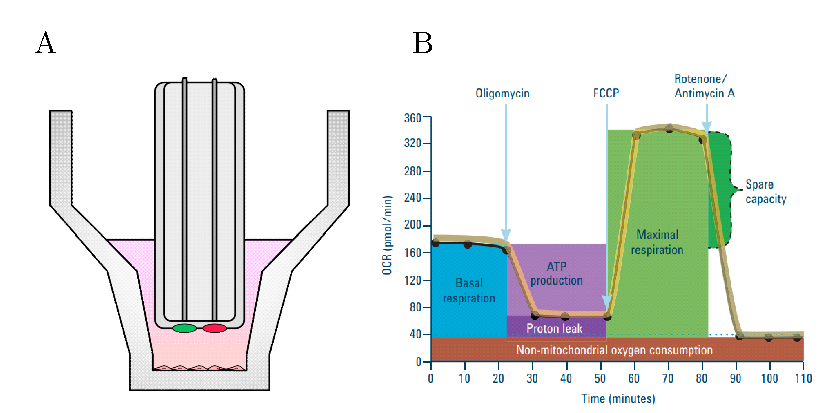
\includegraphics{Abbildung/seahorse_basics_placeholder.pdf}

        \begin{minipage}{\captionwidth}
            \caption[enrichment]{\uzlemph{Basics of Seahorse Assay (a placeholder)}\\
            \textbf{(A)} Schematic of a well-used for Seahorse Assay. For the measurement, the piston in the middle lowers to the bottom, this way defining a restricted space at the bottom. \ac{ocr} and \ac{eacr} in this volume are measured via two probes (red and green). \textbf{(B)} Exemplary curve for \ac{ocr} recorded over time and extractable properties of the respiratory chain.}
            \label{fig:seahorse_basics}
        \end{minipage}
    \end{figure}

    Cells were quantified using a python script provided by Dr. Tobias Reinberger. \ac{ocr} and \ac{ecar} were calculated by the XF Analyzer and normalized using the cell count and the signal in the control wells. In total, three biological repeats were recorded. One of which was excluded because no changes in \ac{ocr} and \ac{ecar} could be detected and cells detached from the bottom of the wells during staining. For the remaining two replicates, the least fitting of the 5 technical repeats for each condition was manually excluded. Further, initial \ac{ocr} and \ac{ecar}, as well as the characteristics of the respiratory chain displayed in figure \ref{fig:seahorse_basics} B, were calculated, using a modified python script provided by Dr. Tobias Reinberger. Assuming a normal distribution, a student's t-test was used, and a p-value of 0.05 is considered significant. For detailed information, please refer to the script.

\section{Oxidative Stress Assay}
\label{sec:cellrox}
CellROX\texttrademark~Green is a fluorescent dye that gets oxidized in an environment of oxidative stress and then binds to DNA, showing bright-green fluorescence \cite{thermofisherscientificinc.CellROXGreenReagent}.
CellROX\texttrademark~Green assay was used to assess generation of \ac{ros} in \acp{haosmc} differentiated as described in section \ref{subsec:differentiation}. After differentiation, further stimulation (from here on referred to as \textit{boost}) with \ac{pdgf} was carried put. Finally, a recovery experiment was performed using \ac{nac}, a potent antioxidant, to quench generation of \ac{ros}.

    \subsection{CellROX\texttrademark~Assay}
    For the assay, cells were washed with \ac{pbs}, then the boost was performed using variable concentrations of \ac{pdgf} in 300\,µL \ac{hbss}. For \ac{ros} quenching with \ac{nac}, 0.25\,M \ac{nac} solution was added to the wells 2\,h prior to the experiment and also added to \ac{hbss} during the experiment.

    \begin{table}[h]
    \capstart
    \centering
    \begin{minipage}{\captionwidth}
        \caption[Seahorse Assay]{\uzlemph{Composition for Seahorse Assay Boost}}
        \label{tab:cellrox_table}
    \end{minipage}
    \begin{tabular}{|c|c|c|c|}
        \hline
        component         & concentration & final concentration      & volume (µL) \\ \hline
        HBSS              & -             & -                        & 300         \\
        PDGF              & 100\,µg/mL             & variable (0\,-\,400\,ng/mL) & variable    \\
        Hoechst           & 1\,mg/mL       & 1\,µg/mL                  & 0.3         \\
        CellROX\texttrademark~Green (1:500) & 2.5\,mM        & 5\,µM                     & 0.6         \\
        NAC               & 0.25\,M        & variable (0\,-\,8\,mM)      & variable    \\ \hline
        total             & -             & -                        & $\sim$300   \\ \hline
    \end{tabular}
    \end{table}

    Cells were kept at 37°C in a 5\,\% CO2 environment during the boost, the incubation time is indicated with the results of the respective experiment. Imaging was done with the BZ-X810 All-in-One Fluorescence Microscope, using standard sensitivity. Images for the \ac{nac} quench were recorded as a z-stack and merged into one image using [KEYENCE SOFTWARE].

    \subsection{Processing of Data}
    \label{subsec:cellrox_data_processing}
    For \ac{pdgf}-boost titration, 7 biological repeats were performed, of which one was excluded because of a high signal in the negative control. For \ac{nac} quench, 4 biological repeats were performed, of which one has been excluded because no signal in the positive control.
    For quantification of signal intensity, pixels with a green value higher than 90 were counted. Differences in cell count were adjusted by division through the number of pixels with a blue value bigger than 80. To adjust for the large variance in total signal intensity between biological repeats, values were adjusted by division through the total signal of all recorded conditions.
    For statistical testing, the Mann-Whitney U test was used, and a p-value of 0.05 is considered significant. For detailed information, please refer to the scripts.


\section{Curation of Data for postGWAS Analyses}
\label{sec:database}
Data for postGWAS analyses and co-visualization with the \ac{gwas} data, were downloaded from public resources. Processing of the data and further annotation is briefly described in the following listing. The generated tables are summarized in figure \ref{fig:db_er} and table \ref{tab:db_tables}. For a complete view, please refer to the download scripts.

\begin{itemize}
    \item \uzlemph{GWAS Summary Statistics:} The \ac{cad} \ac{gwas} summary statistics from \textcite{aragamDiscoverySystematicCharacterization2021} as well as a list of identified proxy \acp{snp} from the study were annotated via the Ensembl \ac{rest} \ac{api} by Dr. Tobias Reinberger.

    \item \uzlemph{HGNC Gene List} The newest quarterly update to the complete \ac{hgnc} dataset was downloaded via the \MYhref{http://ftp.ebi.ac.uk/pub/databases/genenames/hgnc/archive/}{\ac{hgnc} \ac{ftp} server}. The dataset was used to generate a list of all 43135 approved symbols, mapping to their \ac{hgnc} ID as well as a list of all 98723 symbols (approved, alias, and previous), mapping to their \ac{hgnc} ID.

    \item \uzlemph{Linked SNPs} \ac{ld} $r^2$ values for variants in a 500 kb window around all variants in the list of \ac{cad} \ac{gwas} proxy variants, were computed and downloaded via the \MYhref{https://rest.ensembl.org/documentation/info/ld_id_get}{ensembl \ac{rest} \ac{api}}. For humans, ensembl calculates the \ac{ld} with data from the 1000 Genomes project (see table \ref{tab:populations}). In the same process, linked \acp{snp} were annotated with their most severe consequence from the ensembl \ac{vep}. In total information for 449770 relationships were downloaded.

    \begin{table}[h]
    \capstart
    \centering
    \begin{minipage}{\captionwidth}
        \caption[1000 Genomes Populations]{\uzlemph{1000 Genomes Populations}}
        \label{tab:populations}
    \end{minipage}
    \begin{tabular}{|c|c|c|}
        \hline
        Name                   & Size (individuals)   & Description      \\ \hline
        1000GENOMES:phase3:ALL & 2504                 & All phase 3 individuals  \\
        1000GENOMES:phase3:AMR & 347                  & Americans  \\
        1000GENOMES:phase3:EAS & 504                  & East Asians  \\
        1000GENOMES:phase3:EUR & 503                  & European \\
        1000GENOMES:phase3:SAS & 489                  & South Asian  \\ \hline
    \end{tabular}
    \end{table}

    \item \uzlemph{Ensembl Genome Annotatation} The newest Ensembl build (Ensembl release 106) was downloaded via the \MYhref{http://ftp.ensembl.org/pub/current_gtf/homo_sapiens/}{ensembl \ac{ftp} server}. Features annotated as genes of the type protein-coding (19994), lncRNA (17734), or miRNA (1877) were extracted. Further gene symbols were mapped to their \ac{hgnc} ID if possible.

    \item \uzlemph{Ensembl Regulatory Build} The newest ensembl regulatory build (Ensembl release 106) was downloaded via the \MYhref{http://ftp.ensembl.org/pub/current_regulation/homo_sapiens/}{ensembl \ac{ftp} server}, containing 110623 open chromatin regions, 30873 \ac{tf} binding sites, 175885 \ac{ctcf} bindsing sites, 127935 enhancers, 36597 promotors \& 140548 promotor flanking regions.

    \item \uzlemph{Open Target Genetics l2g Scores} The latest list of Open Target Genetics \ac{l2g} Scores was downloaded via the \MYhref{http://ftp.ebi.ac.uk/pub/databases/opentargets/genetics/latest/l2g/}{open target genetics \ac{ftp} server}. Entries were annotated with their \ac{hgnc} ID whenever possible, 655 entries that do not map to a gene that is approved by the \ac{hgnc} were dropped, yielding a total of 3580206 database entries.

    \item \uzlemph{TSS} 35160 \ac{tss} for protein-coding genes were extracted from a \MYhref{https://ccg.epfl.ch/mga/hg38/gencode/}{\ac{USCS} Genome Browser dump}.

    \item \uzlemph{Associated traits from GWAS catalog} The \ac{snp} trait associations from the latest release of the GWAS catalog as well as the accompanying list of studies were downloaded via the \MYhref{http://ftp.ebi.ac.uk/'}{GWAS catalog FTP server}. 14892 \ac{snp}-trait correlations missing a position on the human reference genome or the p-value for the association were dropped from the data set. Further, the column for Odds Ration or beta was separated into two columns. In total, 370002 associations from 5831 distinct studies were collected.

    \item \uzlemph{TADs} \acp{tad} predicted by software adapted from \textcite{dixonTopologicalDomainsMammalian2012} were downloaded via the \MYhref{http://3dgenome.fsm.northwestern.edu/publications.html}{3D genome browser}. In total, \acp{tad} in 40 distinct biosamples were downloaded.

    \item \uzlemph{scATAC-seq from \textcite{newmanMultipleCellTypes2021a}} Processed sc\ac{atac} data for 8 celltypes [SOME MORE INFO] were scraped from the \MYhref{https://github.com/MillerLab-CPHG/Coronary_snATAC/tree/main/3_SVMpipeline/celltype_peaks}{Miller Lab GitHub repository}.

    \item \uzlemph{scATAC-seq from CATlas} Processed sc\ac{atac} data was scraped from the \MYhref{http://renlab.sdsc.edu/kai/Key_Processed_Data/Peaks/}{Ren Labs website} for 222 biosamples.

    \item \uzlemph{ABC model} The \ac{abc} model data for 131 biosamples was downloaded from the \MYhref{http://ftp.broadinstitute.org/outgoing/lincRNA/ABC/}{Engreitz Lab \ac{ftp} server}. The data was further translated from \ac{hg19} to \ac{hg38} using pyliftover.

    \item \uzlemph{ENCODE cCREs} \acp{cCRE} in distinct biosamples were downloaded by Dr. Tobias Reinberger, filtering out elements that were annotated as \textit{unclassified}.
\end{itemize}

\section{Visualization of GWAS data}
\label{sec:gwas_vis}
For visualization of the data, a bokeh application was built, that fetches the data from the database and renders it to a web browser.\\
Bokeh is a python module that allows easy and interactive visualization of data. It combines the powerful data processing tools of python with the interactivity of JavaScript running in the browser. The python side of bokeh creates python objects which are serialized into \ac{json} data and handed over to bokehJS which deserializes them into JavaScript objects that are rendered to the browser. The integrated bokeh server additionally offers the possibility to synchronize data between the underlying python environment and browser-side JavaScript library, allowing real-time updates to the displayed data.

    \begin{figure}[h]
    \capstart
        \centering
    	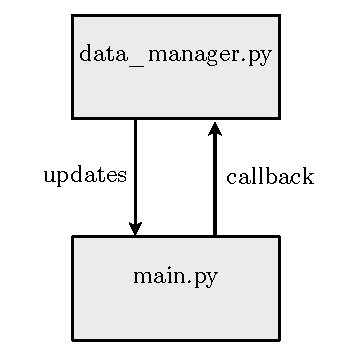
\includegraphics{Abbildung/vis_architecture.pdf}

    	\begin{minipage}{\captionwidth}
    		\caption[vis archi]{\uzlemph{Architecture of the GWAS Navigator}}
    		\label{fig:plot_architecture}
    	\end{minipage}
    \end{figure}

According to good design principles, the concerns of the application are split into two sections, as shown in fig. \ref{fig:plot_architecture}. Reading of data from the database and further processing steps are managed by a data provider and enclosed in one class. In contrast to the model-controller-view architecture, a popular architectural pattern for the design of user interfaces, there is no partition between a view and a controller. Since data visualization, as well as the control widgets, are created by bokeh, it is convenient to use the built-in event listeners of the library to handle the required callbacks. Therefore, the main file is responsible for the creation of all plots and widgets as well as listening for inputs.

\section{Enrichment analysis}
\label{sec:enrichment}
Based on the data in the database, initial postGWAS studies were run. Annotation enrichment analyses are a popular tool for the identification of terms that are over-represented in a list of interest. The most prominent application is their application as \ac{gsea}. \Acp{gsea} are used to check for the overrepresentation of a candidate gene list in a predefined set of genes \cite{tipneyIntroductionEffectiveUse2010}. In this case, the method is used to determine if \acp{cCRE} overlaps with \ac{cad} associated \acp{snp} is enriched in certain biosamples, using Fisher's exact test.\\
For the analysis, \acp{cCRE} annotated as unclassified were excluded. As a list of \ac{cad} associated \acp{snp} the list of 241 proxy variants from the database was used, as well as all linked variants ($r^2\geq0.6$) in the 1000 Genomes European Population. The following parameters were calculated for all biosamples:

\begin{itemize}
    \item The number of distinct cCREs among all biosamples (m)
    \item The number of distinct cCREs that are annotated in the biosample of interest (mt)
    \item The Number of distinct cCREs that overlap with an SNP in the SNP list in any biosample (n)
    \item The Number of distinct cCREs that overlap with an SNP in the SNP list in the biosample of interest (nt)
\end{itemize}

The p-value for the number of overlaps to be greater than or equal to the observation can be calculated as the cumulative distribution function of the hypergeometric distribution.

$$ P(\sigma_t\geq n_t) = \sum_{k=n_t}^{min(m_t, n)} \frac{\binom{n}{k}\binom{m-n}{m_t-k}}{\binom{m}{m_t}} $$

To account for the multiple comparisons problem, p-values were adjusted with Bonferroni correction where n is the number of tests ($\equiv$ number of biosamples):

$$ p_{ajd.} = p*n$$

The analysis and visualization were done in python. An adjusted p-value of 0.05 is considered significant. Finally, the identified biosamples were annotated via the \MYhref{https://web.expasy.org/cellosaurus/}{cell line database Cellosaurus}. For detailed information, please refer to the analysis scripts.

\begin{figure}[h]
\capstart
    \centering
    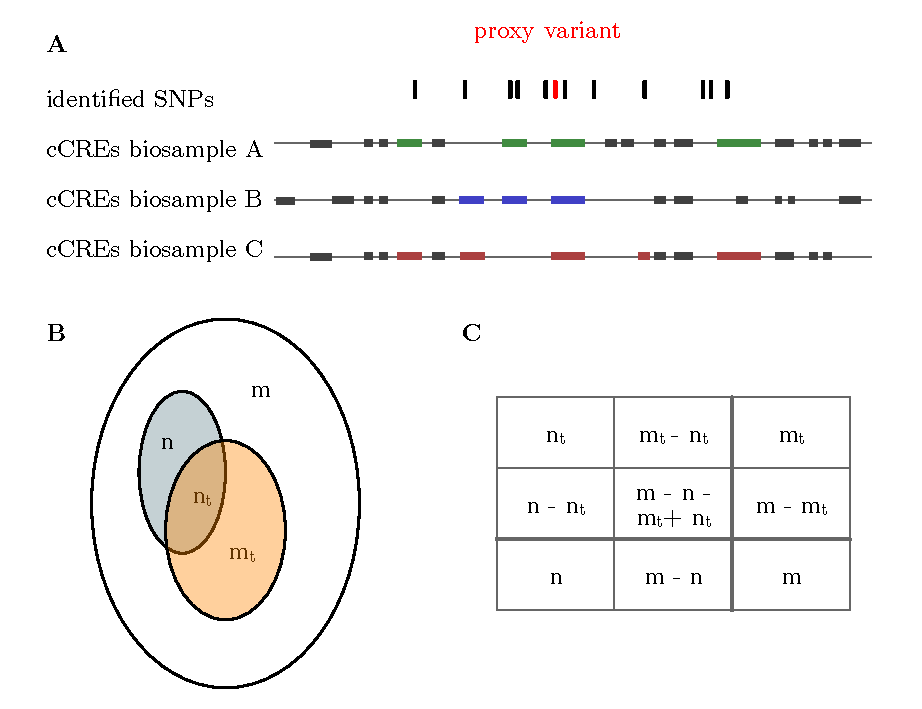
\includegraphics{Abbildung/enrichment.pdf}

    \begin{minipage}{\captionwidth}
        \caption[enrichment]{\uzlemph{Enrichment analysis for \acp{cCREs} overlapping with \ac{cad} risk \acp{snp}}\\
        \textbf{(A)} Visual representation of the overlap calculation for enrichment calculation. The proxy variant is indicated as a red line, variants in \ac{ld} are indicated as black lines. \ac{cCRE} are shown as boxes, those that are overlapping with an \ac{snp} were colored according to the biosample they were annotated in. \textbf{(B)} Venn diagram of these values for a biosample. \textbf{(C)} Schematic contingency table for a biosample. \\
        (m) is the number of distinct \acp{cCRE} found among all biosamples (23 in this example); (mt) the number of distinct \acp{cCRE} annotated in the biosample of interest (16 for biosample A, 14 for biosample b, 14 for biosample C); (n) the number of distinct \acp{cCRE} overlapping with an \ac{snp} (6 in this example);  the number of distinct \acp{cCRE} overlapping with an \ac{snp} in the biosample of interest (4 for biosample A (green), 3 for biosample B (blue), 5 for biosample C (red))}
        \label{fig:enrichment}
    \end{minipage}
\end{figure}
